% 01_first_manuscript.tex
\chapter{第一篇手稿}
\label{chap:hello_world}

我们假设你已经安装好了 \TeX 系统,现在我们来看一下你接触到的第一份 \LaTeX{} 代码。

\section{代码和解释}

\begin{lstlisting}[style = lltx, caption = {Hello \LaTeX{}}, label = {lst:hello}]
\documentclass[a4paper, 12pt]{article}
\title{My First Manuscript}
\author{Liam Huang}
\date{\today}
\begin{document}
\maketitle
% This line is left blank intentionally.

Hello \LaTeX. I have a mathematics equation here: $E = mc^2$.
\end{document}
\end{lstlisting}

\lstinline[style = iltx]|\documentclass[a4paper, 12pt]{article}|
是我们接触到的第一个 \LaTeX{} 命令。
所谓 \LaTeX{} 命令,是指源代码中形如
\cs{\meta{命令}}\oarg{可选参数}\marg{必选参数} 的字符串。
它们以一条反斜线 \cs{} 开头,之后跟着一个符号或者一串英文字母;
可以接受若干个参数,其中用花括号包裹的是 \marg{必选参数},
用方括号包裹的是\oarg{可选参数}。这里我们遇到的是
\lstinline[style = iltx]|\documentclass| 命令,它的作用是载入必选参数中指定的%
\emph{文档类},并接受方括号中的可选参数来调整文档类的效果。
这里我们载入的是 \lstinline[style = iltx]|article| 文档类,它将以
\lstinline[style = iltx]|12pt| 的字号,
将内容打印在 \lstinline[style = iltx]|a4paper| 上。

\begin{quote}
  所谓文档类,即是文档的类型。它定义了文档的基本格式,储存在 \file{.cls} 文件当中。
  例如此处使用的 \lstinline[style = iltx]|article| 文档类,就储存在
  \file{article.cls} 当中。载入文档类,其实就是将 \file{.cls} 文件载入内存的过程。

  如果你使用的是 \tl{},那么可以在命令行中执行
  \lstinline[style = ibash]|kpsewhich article.cls|
  找到 \file{article.cls} 的具体为止。
\end{quote}

接下来,我们遇到了 \lstinline[style = iltx]|\title|、
\lstinline[style = iltx]|\author| 和 \lstinline[style = iltx]|\date|
三个命令。显而易见,他们分别是用来设置文章的标题、作者以及写作日期的命令。
注意,遵循\emph{内容与格式分离}的原则,在这三个命令的参数中,我们应当\emph{只}%
填写标题、作者以及日期的实际内容,而不应包含它们的格式(如字体、字号等)。
这些格式设置,应该用额外的方式来控制。

\begin{quote}
  控制文章标题、作者和日期格式的代码,在 \lstinline[style = iltx]|\@maketitle| 中。
\end{quote}

再接着,我们遇到了 \lstinline[style = iltx]|\begin{document}| 命令,它与
\lstinline[style = iltx]|\end{document}| 配对,组成了 \env{document} 环境。
这是 \LaTeX{} 的正文环境,文档所有的内容都应该放在这个环境中。

\begin{quote}
  每个 \LaTeX{} 手稿,都应该用 \lstinline[style = iltx]|\documentclass| 载入
  文档类,并将内容写在 \env{document} 环境当中。

  \lstinline[style = iltx]|\begin{document}| 之前的部分,是\emph{导言区}。
  导言区通常用来做一些对文档格式的设置。
  \lstinline[style = iltx]|\end{document}| 之后的部分,会被 \LaTeX{} 忽略。
\end{quote}

在正文中,我们首先看到 \lstinline[style = iltx]|\maketitle| 命令。
这个命令的作用,是\emph{以既定格式}将文章的标题、作者和日期等内容打印出来。

随后我们看到一行以 \lstinline[style = iltx]|%| 开头的行。
在 \LaTeX{} 中,\lstinline[style = iltx]|%| 是注释符号。
意思是,从 \lstinline[style = iltx]|%| 开始,到 \lstinline[style = iltx]|%| 所在
的行结尾,这部分内容都会被 \LaTeX{} 忽略。而将它们写在手稿里的目的,是提示「人们」这段
代码的作用是什么。

最后,我们的目光看到倒数第二行的内容。这一行的内容,会被 \LaTeX{} 打印出来。
不过,其中还有两个值得一提的地方。其一是 \lstinline[style = iltx]|\LaTeX| 命令。
从这个命令的名字就可以看出,它的作用是打印 \LaTeX{} 这个高低不平的 logo。
其二是用 \lstinline[style = iltx]|$ ... $| 符号包裹起来的质能公式。
因为公式总是\emph{价值连城},所以我们用美元符号将他们包裹起来。

\section{操作和输出}

请将代码清单 \ref{lst:hello} 中的内容,用键盘逐字母地输入进电脑,
并保存在文件中 \file{01\_hello.tex}。
注意,这个习惯很重要:\LaTeX{} 代码应该以 \file{.tex} 结尾。
点击「排版」,以 \XeLaTeX{} 编译,你应该看到如图 \ref{fig:hello} 所示的样子。

\begin{figure}[!htb]
\centering
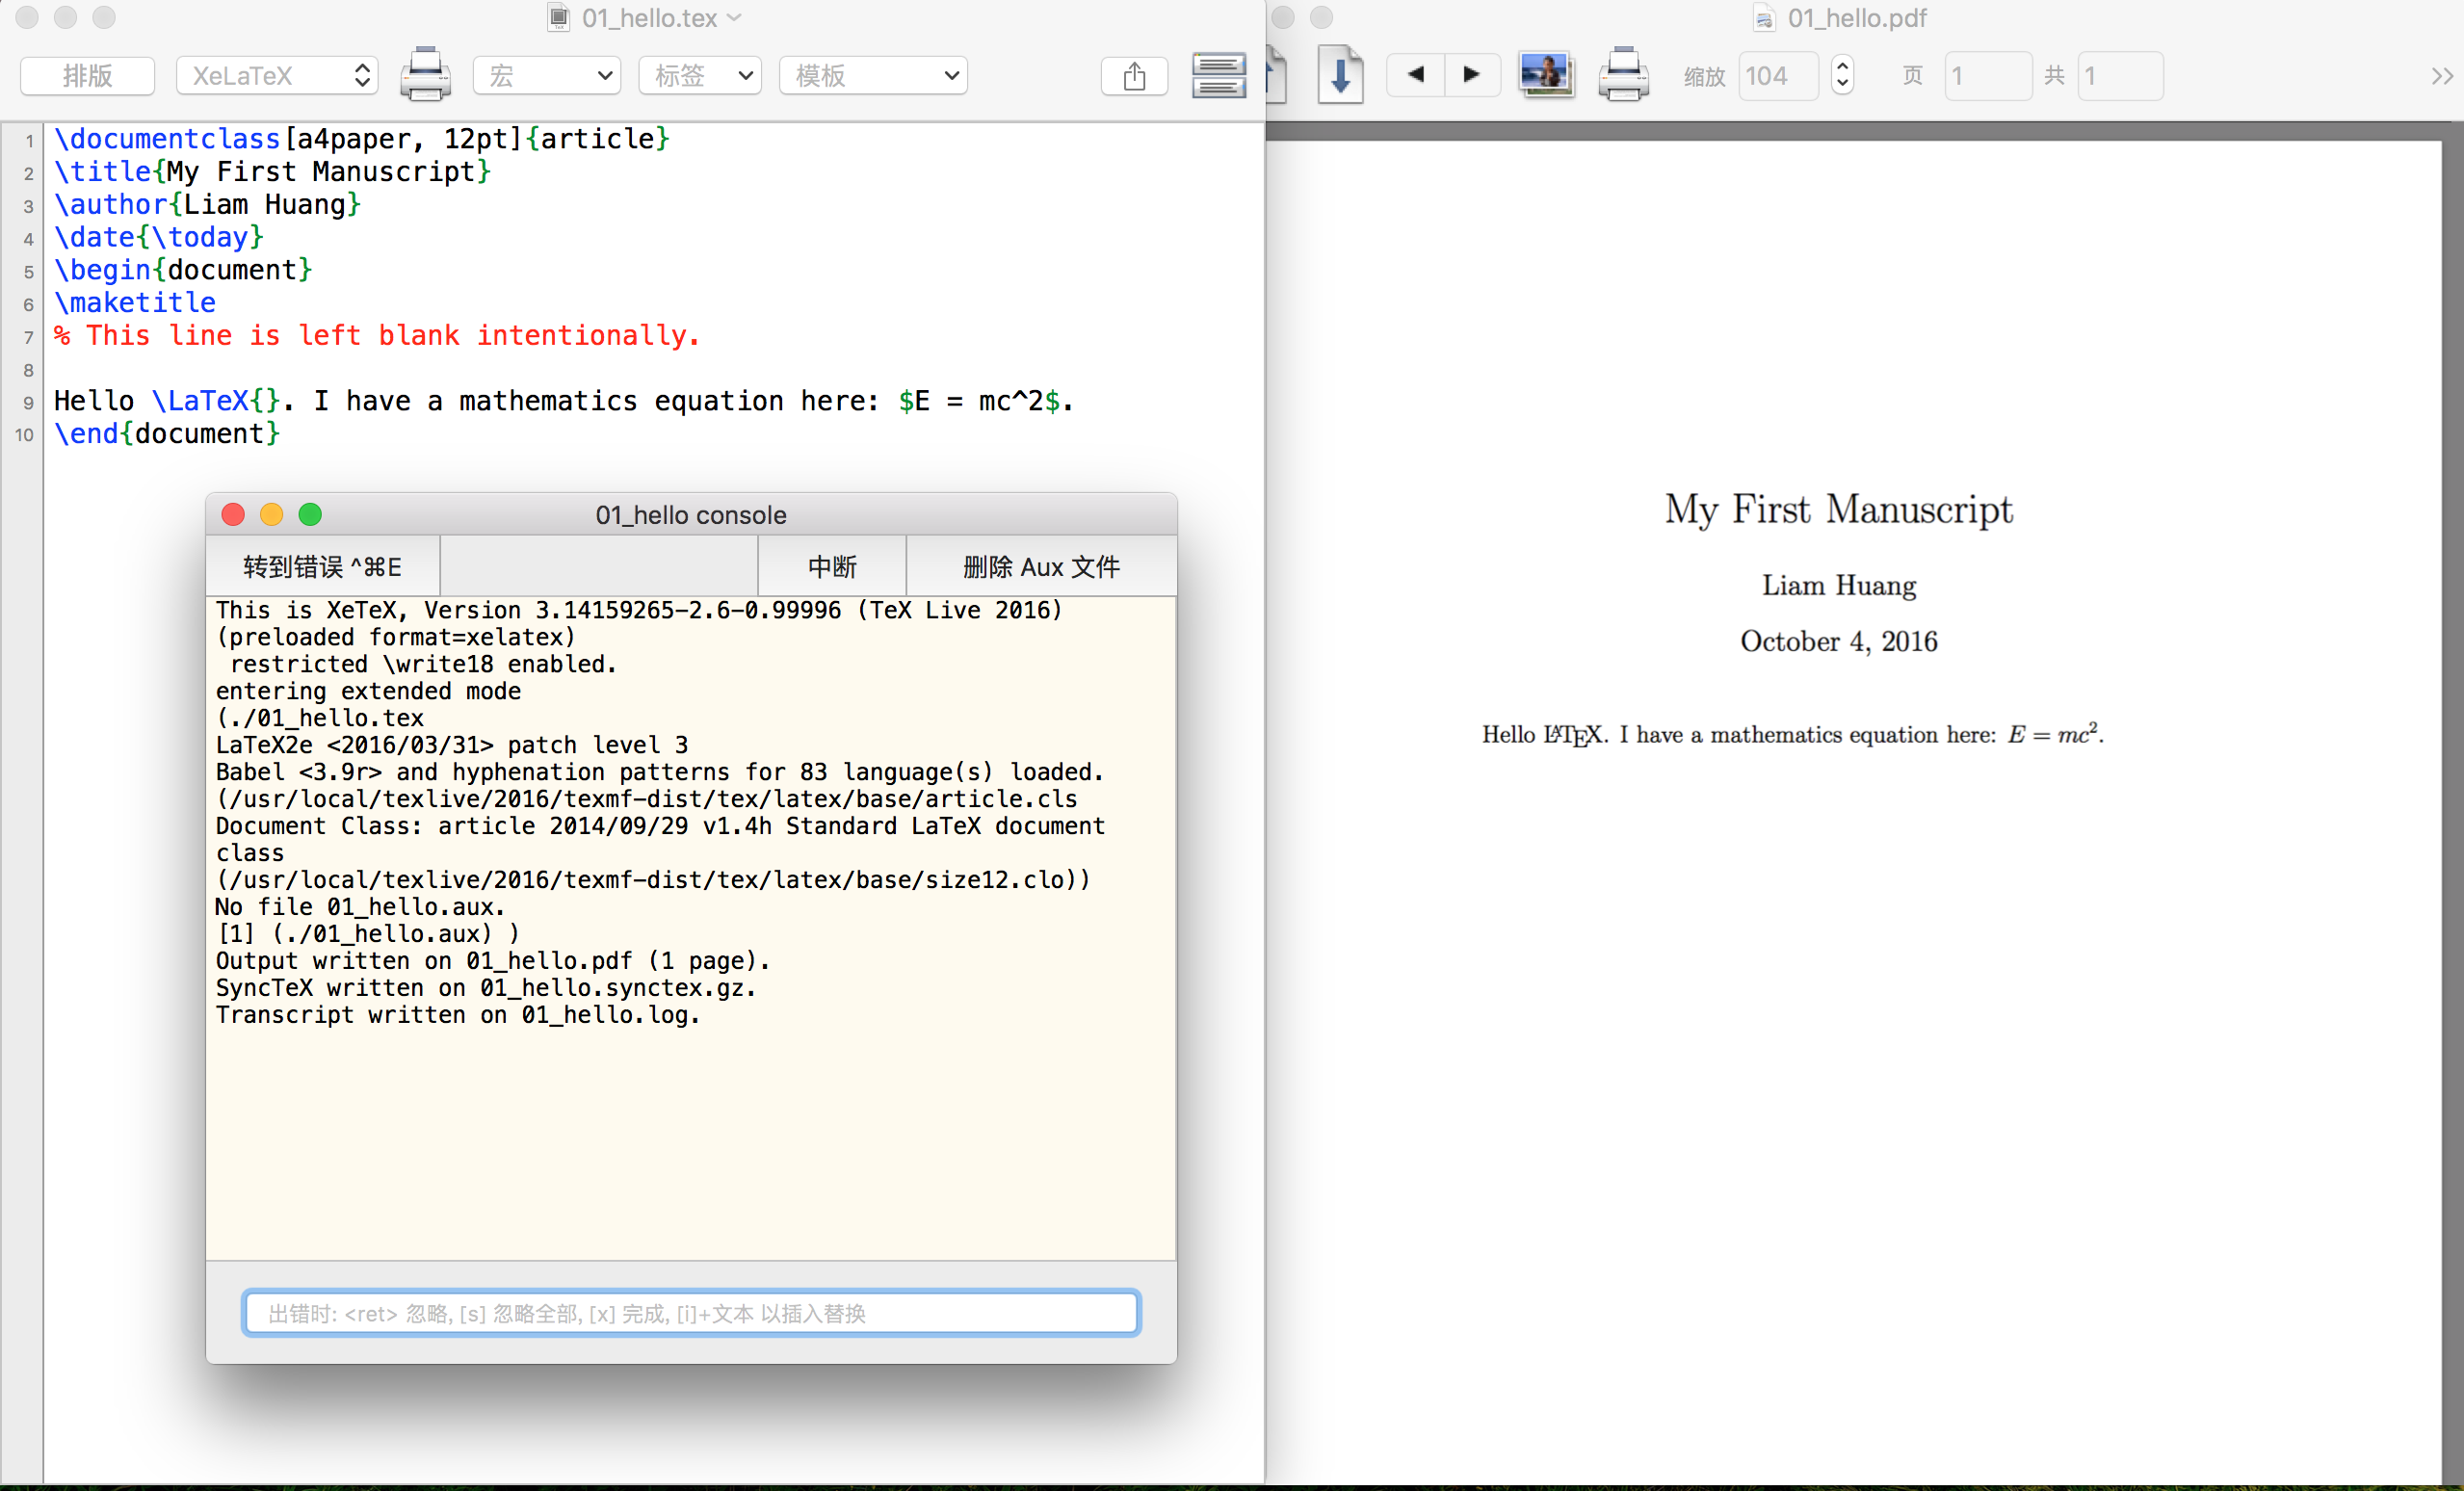
\includegraphics[width = .8\linewidth]{01_hello_mac.png}
\caption{Hello \LaTeX{}}\label{fig:hello}
\end{figure}

如果你看见类似 \ref{lst:hello_wrong} 的输出,这表示你在源代码里写错了一些东西。
请不要慌张,你在学习的过程中会经常遇到类似的问题,最重要的是学会如何阅读错误提示。

\begin{lstlisting}[style = lltx, caption = {错误输出}, label = {lst:hello_wrong}]
! Undefined control sequence.
l.9 Hello \LaTex
                . I have a mathematics equation here: $E = mc^2$.
?
\end{lstlisting}

我们一行一行地看。

\begin{enumerate}
  \item 以一个叹号开头,说明 \LaTeX{} 遇到的错误的名字。这里是「未定义的控制序列」,
  这个错误通常表示你输错了命令,或者使用了一个未经定义的命令。
  \item \lstinline[style = iltx]|l.9| 表示问题出在第九行,
  \lstinline[style = iltx]|Hello \LaTex| 表示 \LaTeX{}
  在处理到这里的时候,遇到了问题。
  \item 第三行是遇到问题时,后续尚未处理的内容。
  \item \LaTeX{} 打印了一个问号,这表示 \LaTeX{} 正在等待我们的输入。
  如果你输入 \lstinline[style = iltx]|x| 则会终止 \LaTeX{} 进程。
\end{enumerate}

这里显而易见,我们将 \lstinline[style = iltx]|\LaTeX| 错误地写作了
\lstinline[style = iltx]|\LaTex|。注意,\LaTeX{} 对命令是区分大小写的。
这里我们将之更正就可以了。

\section{额外习题}

你需要完成这些额外习题,帮助你巩固学到的知识。如果你觉得这部分习题很难,可以先看后面的内容——
但一定要记着回来,解决这些问题。

\begin{enumerate}
  \item 使用搜索引擎(推荐使用 Google),看看 \lstinline[style = iltx]|article|
  文档类还有什么可选参数。修改你的手稿,实际看看这些参数有什么效果。
  \item 删除或者使用 \lstinline[style = iltx]|%| 注释掉
  \lstinline[style = iltx]|\maketitle| 命令,看看会发生什么。思考一下背后的原因。
  \item 尝试打印出更多的内容。
\end{enumerate}

\endinput
